% --
% signal processing

\chapter{Signal Processing and Feature Extraction}\label{sec:signal}
This section describes how to process raw waveforms from audio files to extract meaningful features from them.
Further it is mentioned, how the features are compressed to reduce dimensionality and therefore computational effort for Neural Networks.
In this thesis, either raw audio samples are used directly as features, intended for wavenets, or Mel Frequency Cepstral Coefficients (MFCC) features for all other more classifcal Neural Network Architectures.
At last it is shown what further possibilities exist to enhance MFCC features and create a better visual presentation for them.

% --
% raw audio

\section{Raw Audio Waveforms}\label{sec:signal_raw}
\thesisStateReady
Physical acoustic waves are recorded by microphones, translating mechanical vibrations to electrical signals. 
Those electrical signals are further stored in \emph{waveform files} or \emph{audio files} with a specific audio format, for example the \texttt{.wav} format.
Apart from any compression technique the most important storage details are the bit resolution, e.g. \SI{24}{\bit} floating point and the sample rate $f_s$. 
The sample rate tells, which frequency range of the continuous acoustic waveform is possible to store in a discrete representation.
This is restricted by the Nyquist-Shannon sampling theorem, where the maximal frequency of the signal $f_{x_{max}}$ should not exceed the half of the sampling frequency: 
\begin{equation}\label{eq:signal_raw_nyquist}
  f_{x_{max}} < \frac{fs}{2}
\end{equation}
to prevent aliasing effects.
That is the reason, why the compact disc (CD) format has a sampling frequency of \SI{44.1}{\kilo\hertz} resulting in a maximum signal frequency of \SI{22.05}{\kilo\hertz}, using the fact that humans do not hear above \SI{20}{\kilo\hertz} frequencies.
However it is also possible to go far beyond those \SI{44.1}{\kilo\hertz}, for instance used in telephone systems, where the sampling rate is \SI{8}{\kilo\hertz}.
It is possible to reduce the sampling rate, because voice does not need such a high sampling frequency to have sufficient quality and being understandable.
Music on the other hand requires a high sampling frequency for being enjoyable to listen to.

With the sampling frequency known, a discrete time signal of an audio recording $x \in \R^n$ can be expressed in vector notation:
\begin{equation}\label{eq:signal_raw_x}
  x = [x_1,\, x_2,\, \dots,\, x_n]^T
\end{equation}
with a total number of $n$ samples.
The recorded audio files provided in the speech command dataset \cite{Warden2018} used for the experiments in \rsec{exp}, are sampled with a sampling rate of \SI{16}{\kilo\hertz}, which is totally enough for human speech signals.
Further those recordings usually have a time duration of \SI{1}{\second}, apart from some individual shorter files.

For evaluation and visualization purpose, the author of this thesis recorded his own examples of the speech commands \{\enquote{left}, \enquote{right}, \enquote{up}, \enquote{down}, \enquote{go}\}.
Those showcase examples represent for instance actions in a video game and need to be feature extracted before they are classified with a neural network.
The example are shown in \rfig{signal_raw_showcase} in raw audio format.
\begin{figure}[!ht]
  \centering
    \subfigure[left]{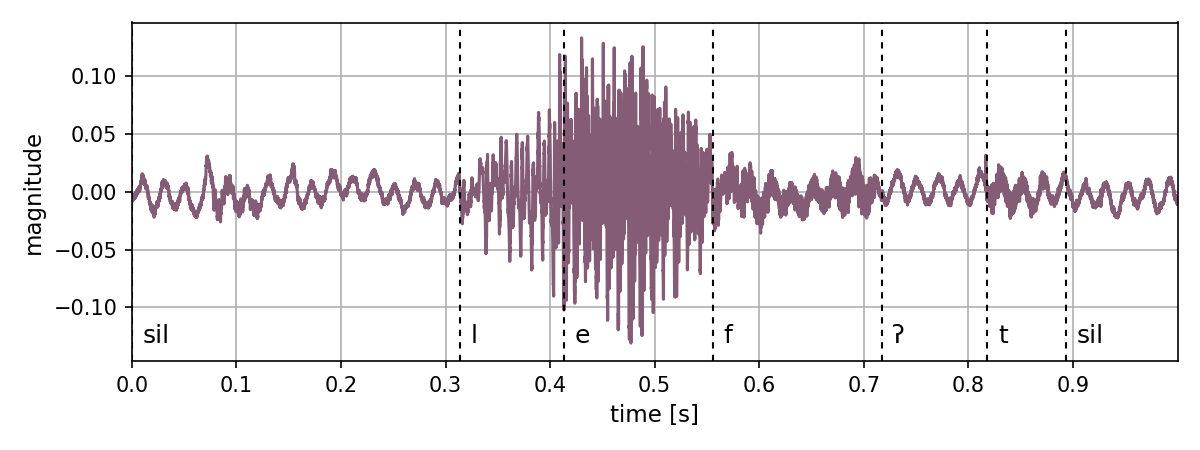
\includegraphics[width=0.45\textwidth]{./3_signal/figs/signal_raw_showcase_left0}}
    \subfigure[right]{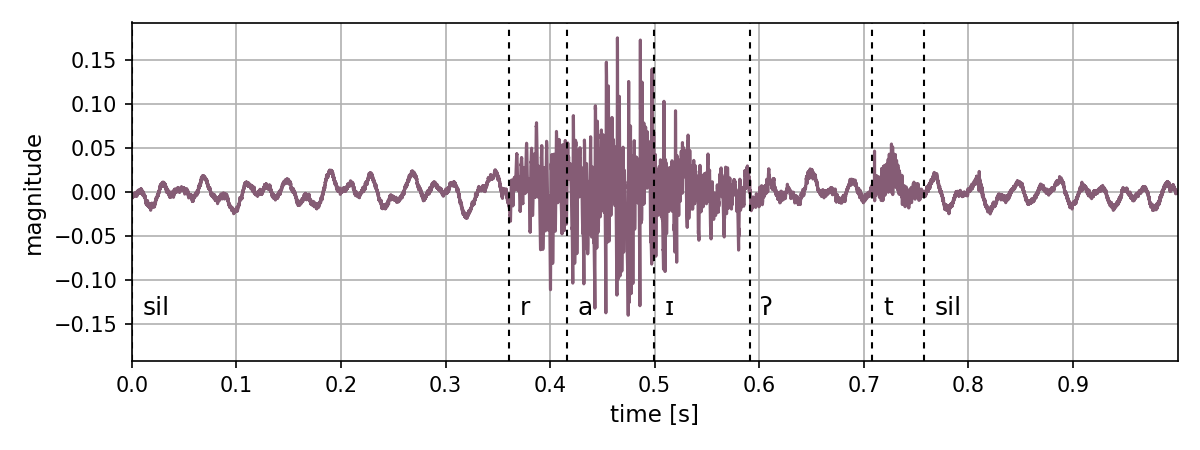
\includegraphics[width=0.45\textwidth]{./3_signal/figs/signal_raw_showcase_right0}}
    \subfigure[up]{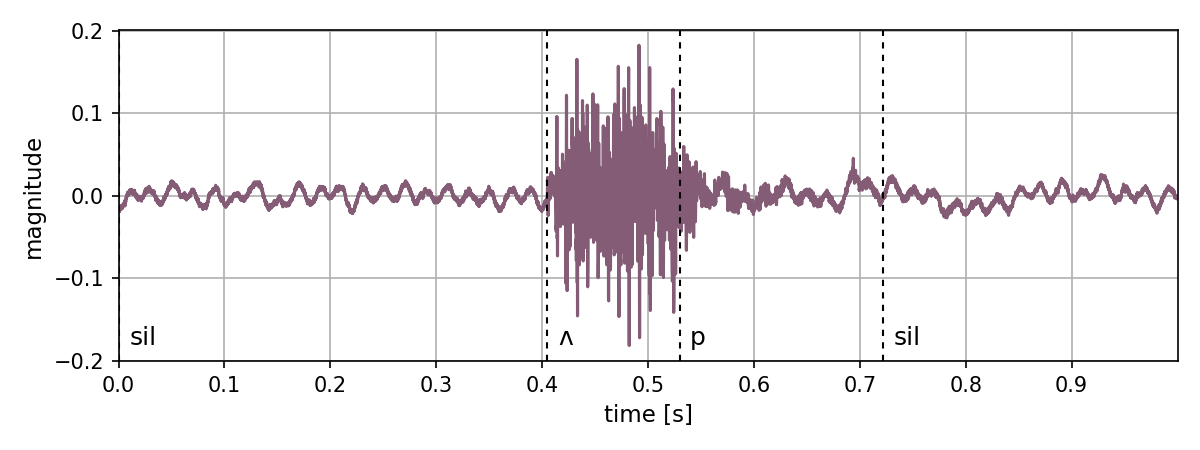
\includegraphics[width=0.45\textwidth]{./3_signal/figs/signal_raw_showcase_up0}}
    \subfigure[down]{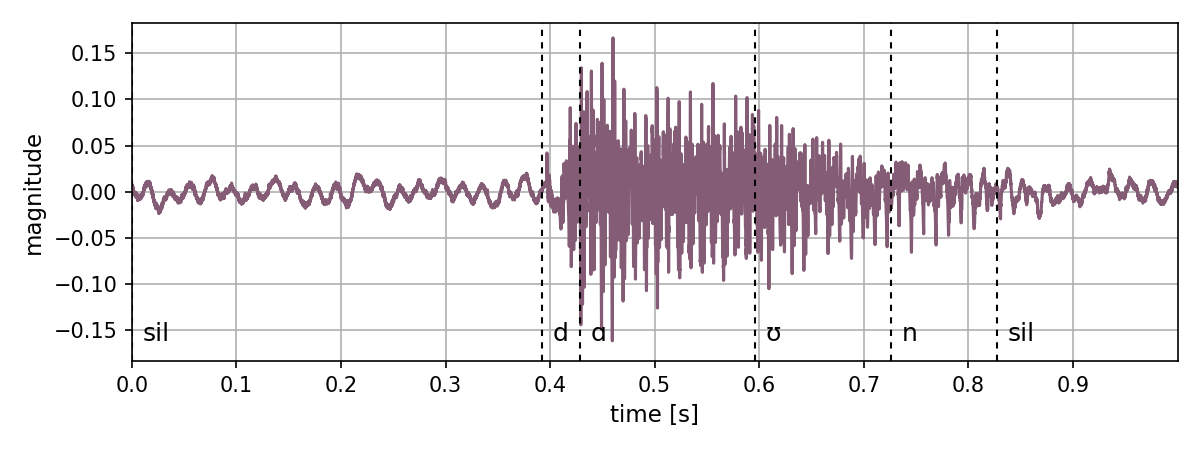
\includegraphics[width=0.45\textwidth]{./3_signal/figs/signal_raw_showcase_down0}}
    \subfigure[go]{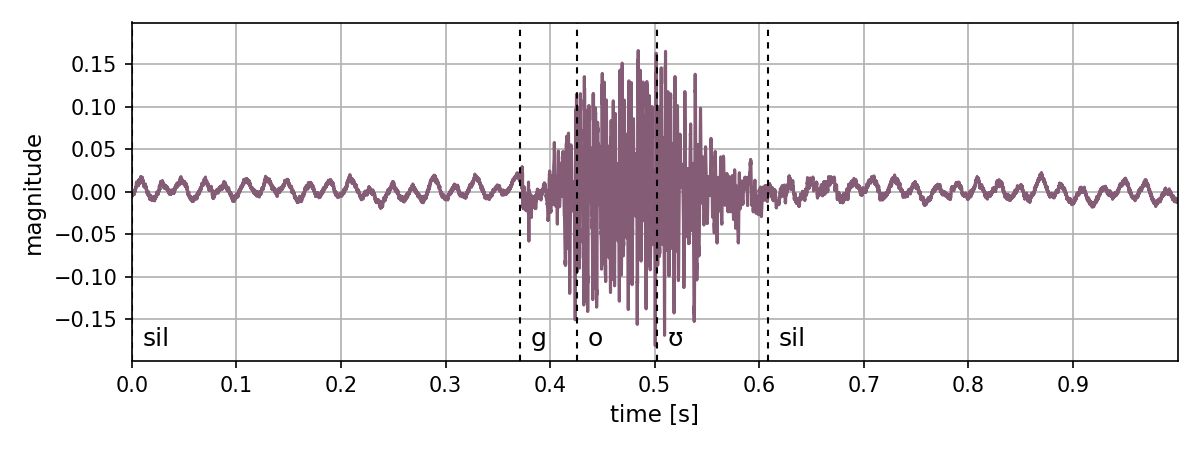
\includegraphics[width=0.45\textwidth]{./3_signal/figs/signal_raw_showcase_go0}}
  \caption{Raw audio waveform files, recorded by the author of this thesis with a simple consumer lavalier microphone.}
  \label{fig:signal_raw_showcase}
\end{figure}
\FloatBarrier
\noindent
From the shown raw audio files, one can estimate how long a speech command may take in terms of duration and see that usually a whole second is too much for a single speech command.
The pronunciation of words can of course deviate strongly in duration, but usually when commanding something it is preferred to speak short and well pronounced.
If a time interval of \SI{500}{\milli\second} is used to capture a speech command (this time interval is used in the feature extraction), it might happen that not every phoneme of the spoken words are captured. 
For instance this might happen often for words with glottal stops before consonants, for example the phoneme \enquote{t} in \enquote{left} or \enquote{right}, therefore the input features may only contain information of the first phonemes \enquote{lef} or \enquote{righ}.
But since Key Word Spotting (KWS) is restricted in its vocabulary and no similar words are included in the vocabulary, it should be no problem in distinguishing those.

Another important aspect is to detect the onset position of the speech commands on the time axis. 
It is easy to see in \rfig{signal_raw_showcase} where the spoken words are beginning and ending, but usually not all recordings are as clean as those.
There might be a huge noise level or background noise or cut away signals, so that the detection of the right onset position for the \SI{500}{\milli\second} time interval within the \SI{1}{\second} recordings is not always appropriate.
An intuitive method is to simply use the signal energy to determine the onset of the key words.
If the signal $x$ is windowed with the length of a \SI{500}{\milli\second} striding frame with sample length $N$, the energy of each windowed signal is calculated with:
\begin{equation}
  e_{w}(m) = \sum_{i=0}^{N-1} \abs{x[i + m]}^2
\end{equation}
with shift index $m = 0 \dots n - N + 1$, where $n$ is the number of sample of $x$.
The onset sample $o$ with the highest energy region is then determined by
\begin{equation}
  o = \underset{m}{\arg \max} \, e_{w}(m)
\end{equation}
for all windowed signal energies $e_{w}(m)$.

At last it should be noted, that the value range in the y-axis of audio recordings strongly depends on the microphone, amplifiers and post processing.
Therefore it is strongly recommended to normalize all recordings to a defined value range, with for instance the infinity norm:
\begin{equation}
  \hat{x} = \frac{x}{\norm{x}_\infty}
\end{equation}
so that the maximum or minimum value corresponds to either $+1$ or $-1$ and the signal range is defined between $[-1, 1]$.
% --
% spectrogram

\section{Spectral Features}\label{sec:signal_spec}
Spectral features, such as a spectrogram, are the most intuitive form to represent audio waveforms. 
It is possible to observe which frequencies are active at time instances.
Methodically this is done by shifting an \emph{analytic window} of time span $t_N$, on the time axis.
The time shifting has also a fixed time interval, denoted as \emph{hop time} $t_{h}$.
Both time parameters $t_N$ and $t_h$ can also be presented in samples by multiplying it with the sampling frequency $f_s$:

% samples
\begin{equation}
  \begin{split}
    N &= t_N \, f_s, \\
    h &= t_h \, f_s.
  \end{split}
\end{equation}
The audio samples contained by the analytic window of size $N$, are transformed with the Discrete Fourier Transform (DFT):

% DTFT
\begin{equation}\label{eq:signal_spec_dtft}
  \tilde{x}[k] = \sum_{n=0}^{N-1} x[n] \, e^{-j\frac{2 \pi n}{N}k}
\end{equation}
into the frequency space $\tilde{x}[k] \in \C$ with frequency index $k$ and discrete audio samples $x[n]$ with sample index $n$.
More conveniently, \req{signal_spec_dtft} can be written in matrix / vector notation with the DFT operator denoted as $\mathcal{F} \in \C^{k \times n}$:

% DFT matrix
\begin{equation}\label{eq:signal_spec_dtft_matrix}
  \tilde{x} = \mathcal{F}\, x \quad \mathrm{with} 
  \quad \mathcal{F}[p, q] = e^{-j\frac{2 \pi p}{N} q},
  \quad p,\, q = 0, 1, \dots k-1,\, 0, 1 \dots n-1.
\end{equation}
where $p$ and $q$ are row and column index in the matrix $\mathcal{F}$.
It follows that $\tilde{x} \in \C^k$ and $x \in \R^n$, where $n$ and $k$ denote here the dimension of input samples and frequency space respectively.

The length of the analytic window in samples $N$ is crucial for the frequency resolution and the lowest frequency that can be represented.
For example, the periodic time of a sound with $f=\SI{20}{\hertz}$ is $t=\frac{1}{f} = \SI{50}{\milli\second}$.
To represent a waveform it is necessary to have at least a quarter of its wavelength captured.
Within this thesis, the length of the analytic window is selected to \SI{25}{\milli\second}.

The other important parameter, the \emph{hop size} in samples of the hop time, by which the analytical window is shifted on the time axis, indicates the resolution in time and is especially important for changes within the audio data.
In applications like speech processing, the hop time should be selected so that the fastest pronounced phone and its transitions to other phones is captured within this time span with sufficient resolution.
Usually a hop time of $t_{h}=\SI{10}{\milli\second}$ is chosen for speech recognition tasks (also used within this thesis), but it could be extended to $t_{h}=\SI{20}{\milli\second}$, demonstrated in like in \cite{Peter2020}, for saving computations.

With those parameters in mind and $h$ denoted as hop size in samples and $N$ the length of the analytical window, the Short-Time Fourier Transform (STFT) for discrete time signals, can be computed as:

% stft
\begin{equation}\label{eq:signal_spec_stft}
    X[m, k] = \sum_{n=0}^{N-1} x[n + m] \, w[n] \, e^{-j\frac{2 \pi n}{N}k}, \qquad m = 0 \cdot h, \, 1 \cdot h, \, \dots, \, M \cdot h 
\end{equation}
note that $n$ is here the summation index, $w$ is a window function, such as the \emph{Hanning} window, $m$ indicates the hop index and $M$ is the maximum number of hops.
The maximum number of hops $M$ are all shifts of the analytic window by the hop size on the discrete time axis and can be computed as:

% hop
\begin{equation}\label{eq:signal_spec_hop}
  M = \frac{n-N}{h}
\end{equation}
where $n$ is here the length of the discrete time signal $x$.
A summary of the STFT parameters are shown in \rtab{signal_spec_stft}.

% stft params
% --
% stft params
\begin{table}[ht!]
\begin{center}
\caption{Parameters used for the STFT computation.}
\begin{tabular}{ M{4cm}  M{4cm}}
\toprule
\textbf{Parameter} & \textbf{Value} \\
\midrule
Sampling Frequency & \SI{16}{\kilo\hertz}\\
Analytic window size & \SI{25}{\milli\second}\\
Hop size & \SI{10}{\milli\second}\\
Window Function & Hanning\\
\bottomrule
\label{tab:signal_spec_stft}
\end{tabular}
\end{center}
\end{table}
\FloatBarrier
\noindent

A spectrogram $P \in \R^{m \times k}$ is simply the power spectrum of the STFT signal and is computed with:

% spec
\begin{equation}\label{eq:signal_spec_spec}
  P[m, k] = \abs{X[m, k]}^2.
\end{equation}
A spectrogram with linear representation is shown in \rfig{signal_spec_lin_examples}.

\begin{figure}[!ht]
  \centering
    \subfigure[left]{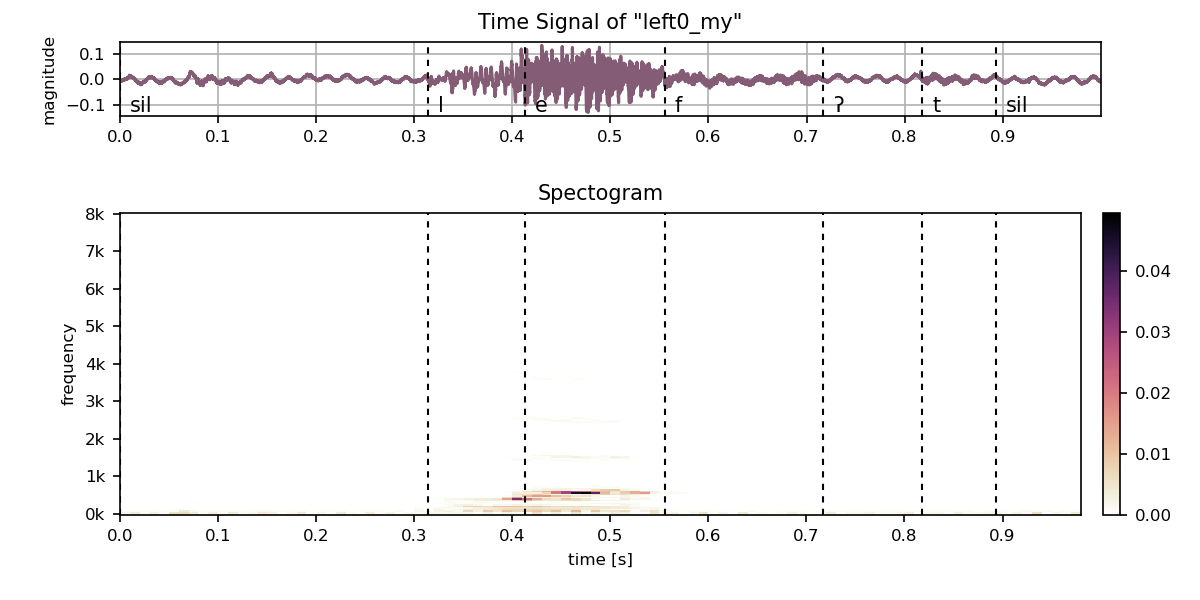
\includegraphics[width=0.45\textwidth]{./3_signal/figs/signal_spec-lin_left0_my}}
    \subfigure[right]{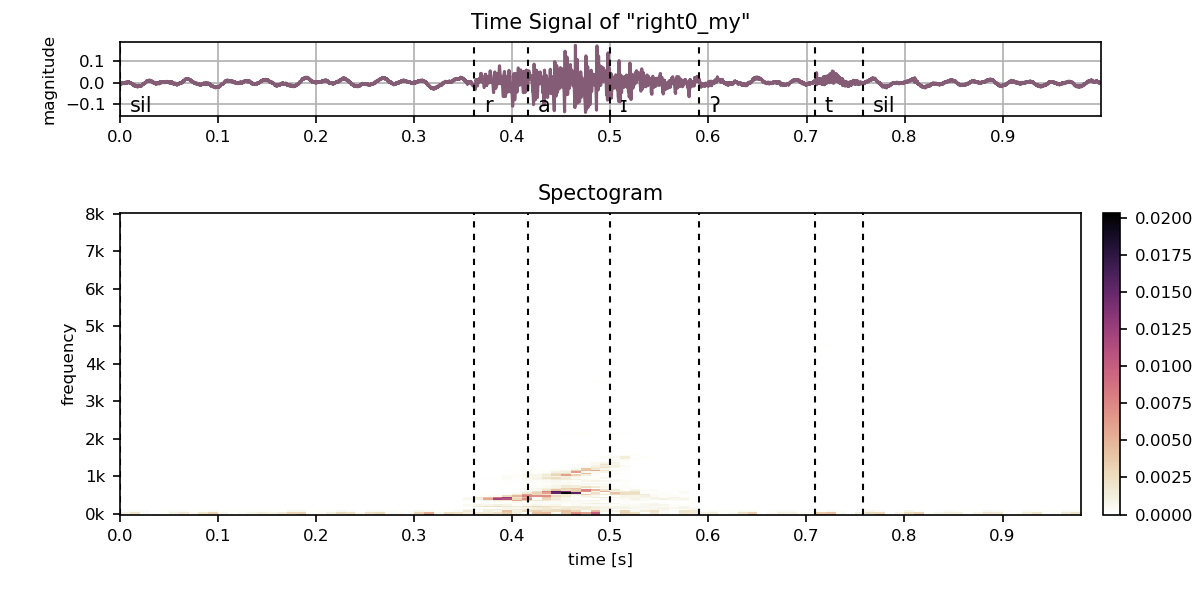
\includegraphics[width=0.45\textwidth]{./3_signal/figs/signal_spec-lin_right0_my}}
    \subfigure[up]{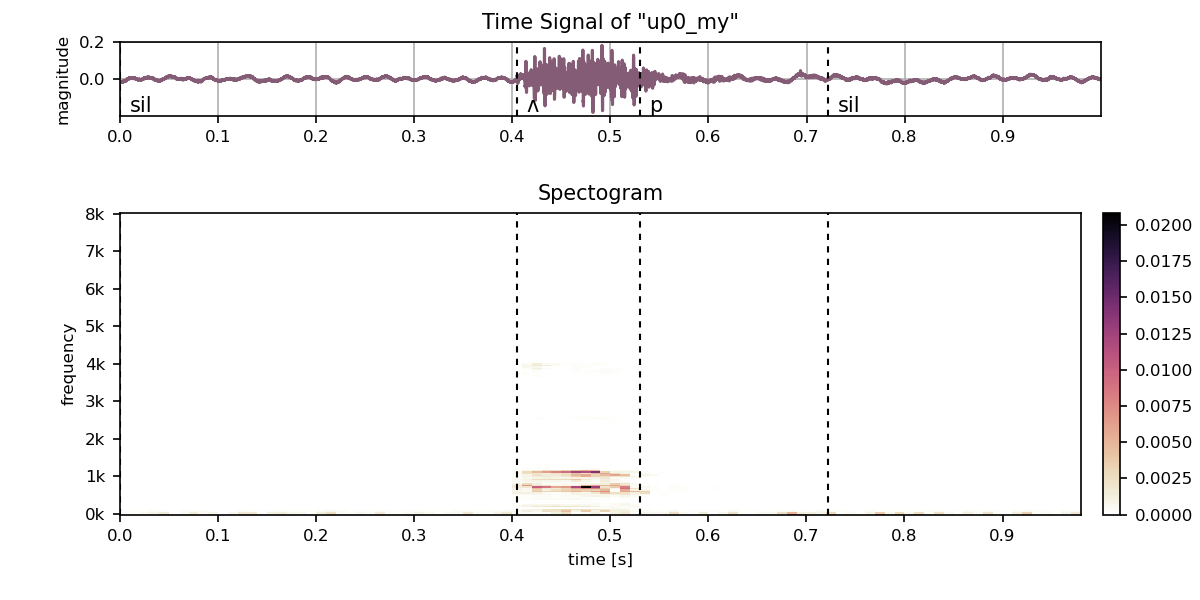
\includegraphics[width=0.45\textwidth]{./3_signal/figs/signal_spec-lin_up0_my}}
    \subfigure[down]{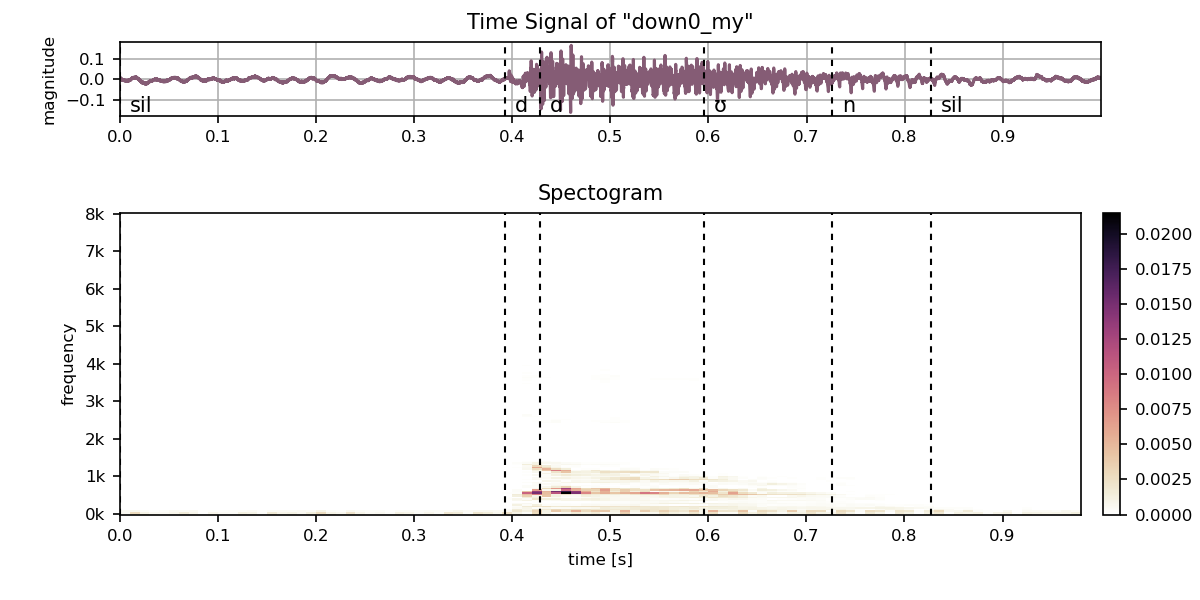
\includegraphics[width=0.45\textwidth]{./3_signal/figs/signal_spec-lin_down0_my}}
    \subfigure[go]{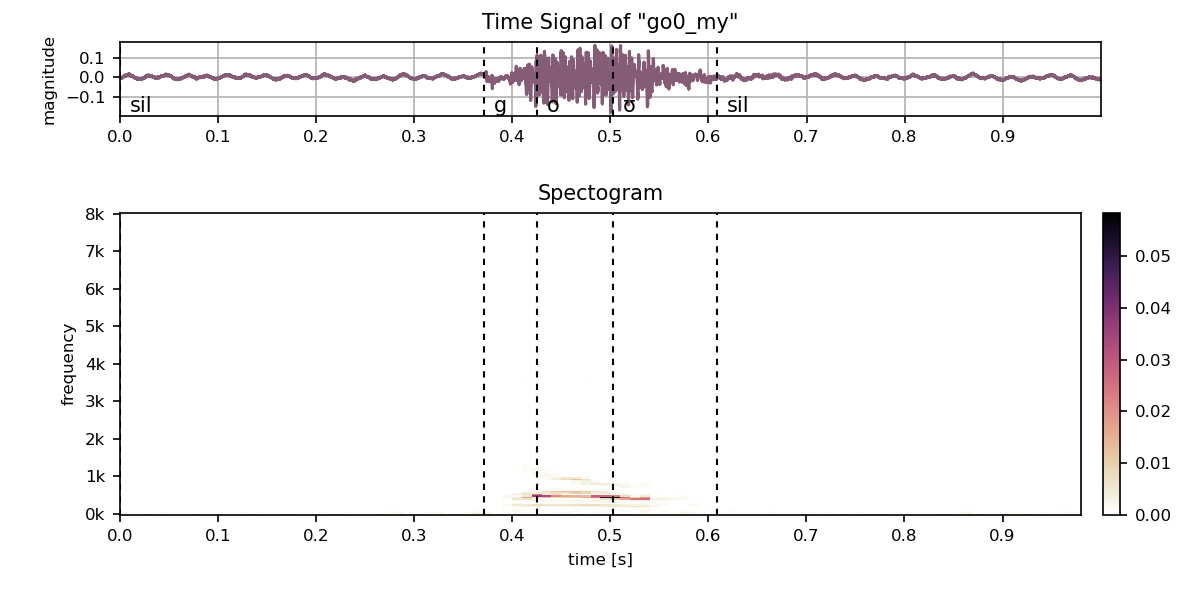
\includegraphics[width=0.45\textwidth]{./3_signal/figs/signal_spec-lin_go0_my}}
  \caption{Spectrogram linear scaled.}
  \label{fig:signal_spec_lin_examples}
\end{figure}
\FloatBarrier
\noindent

One can see here, that most of the energy of the signal is in the lower frequency regions under \SI{1}{\kilo\hertz}.
It is more interesting to transform the signal into the log scale with:

% log
\begin{equation}\label{eq:signal_spec_log}
  P_{DB}[m, k] = 10 \cdot \log{P[m, k]}
\end{equation}
so that small energies are visualized much better. 
The same examples with log scale are shown in \rfig{signal_spec_log_examples}.

\begin{figure}[!ht]
  \centering
    \subfigure[left]{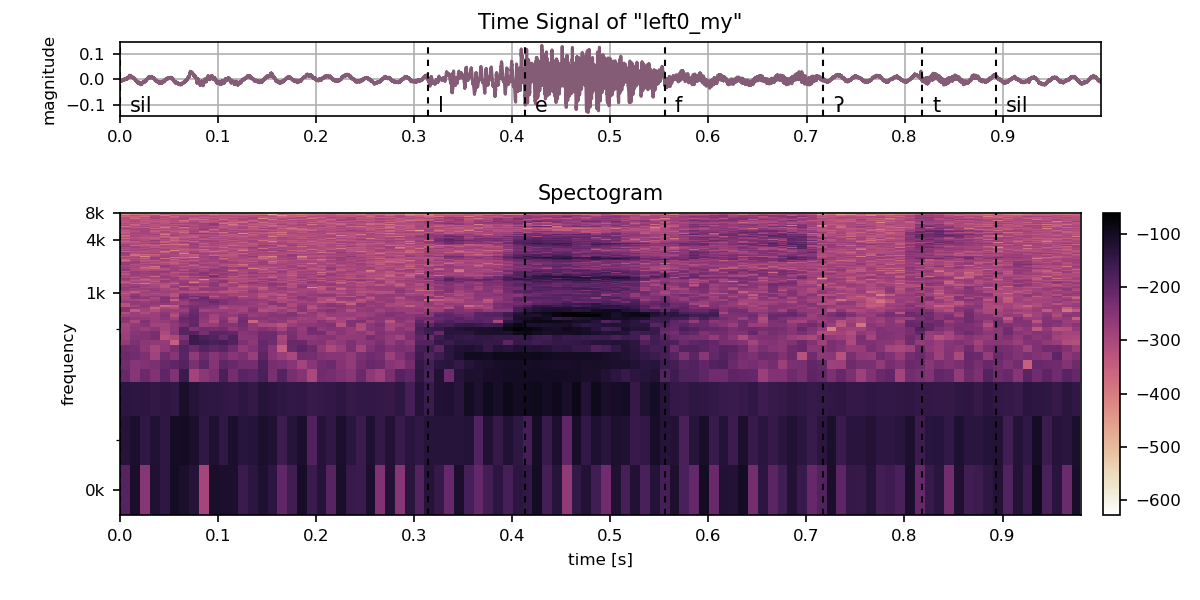
\includegraphics[width=0.45\textwidth]{./3_signal/figs/signal_spec-log_left0_my}}
    \subfigure[right]{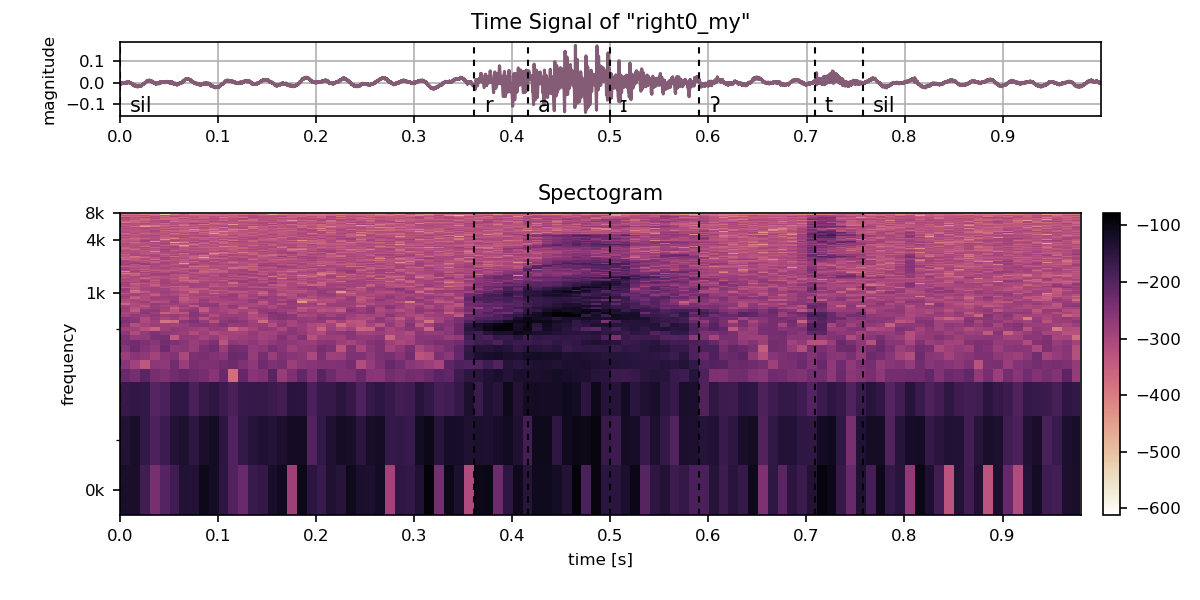
\includegraphics[width=0.45\textwidth]{./3_signal/figs/signal_spec-log_right0_my}}
    \subfigure[up]{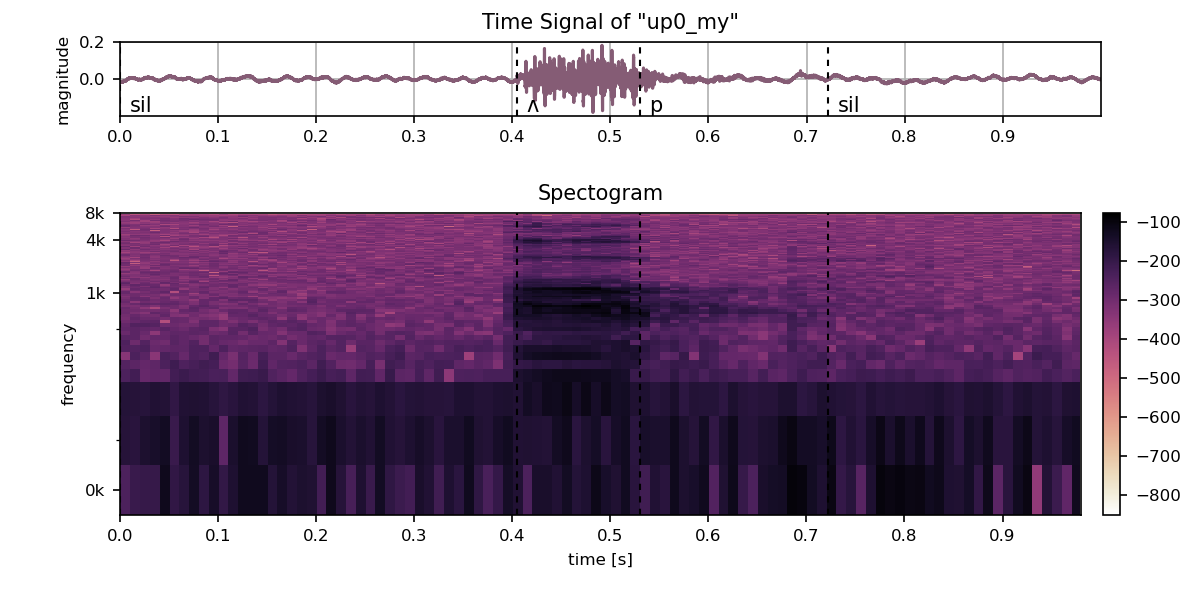
\includegraphics[width=0.45\textwidth]{./3_signal/figs/signal_spec-log_up0_my}}
    \subfigure[down]{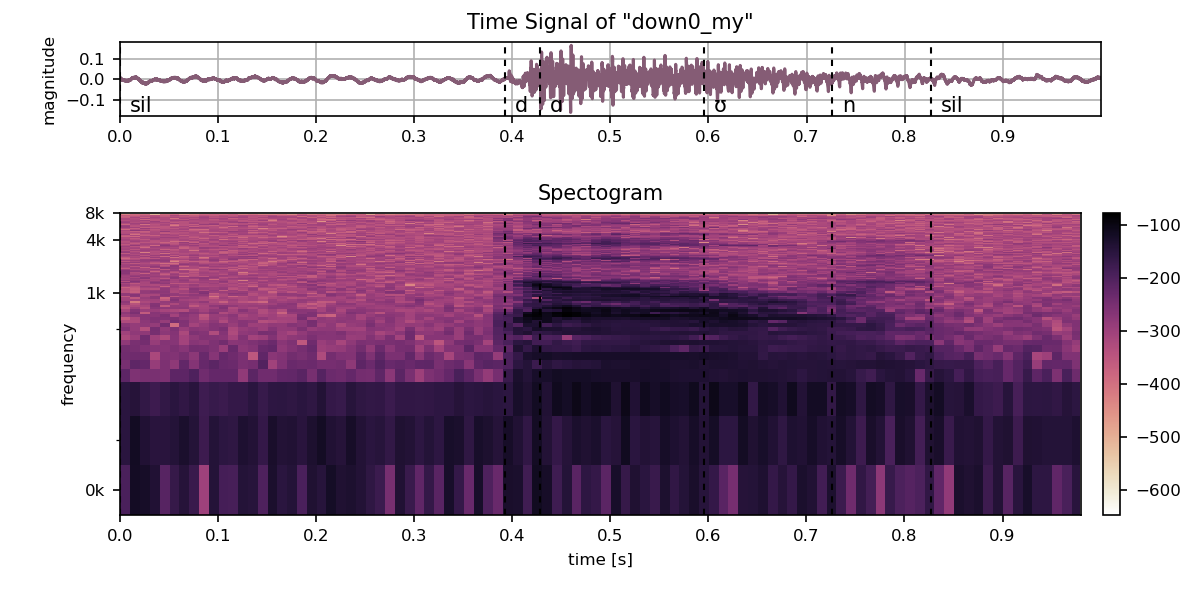
\includegraphics[width=0.45\textwidth]{./3_signal/figs/signal_spec-log_down0_my}}
    \subfigure[go]{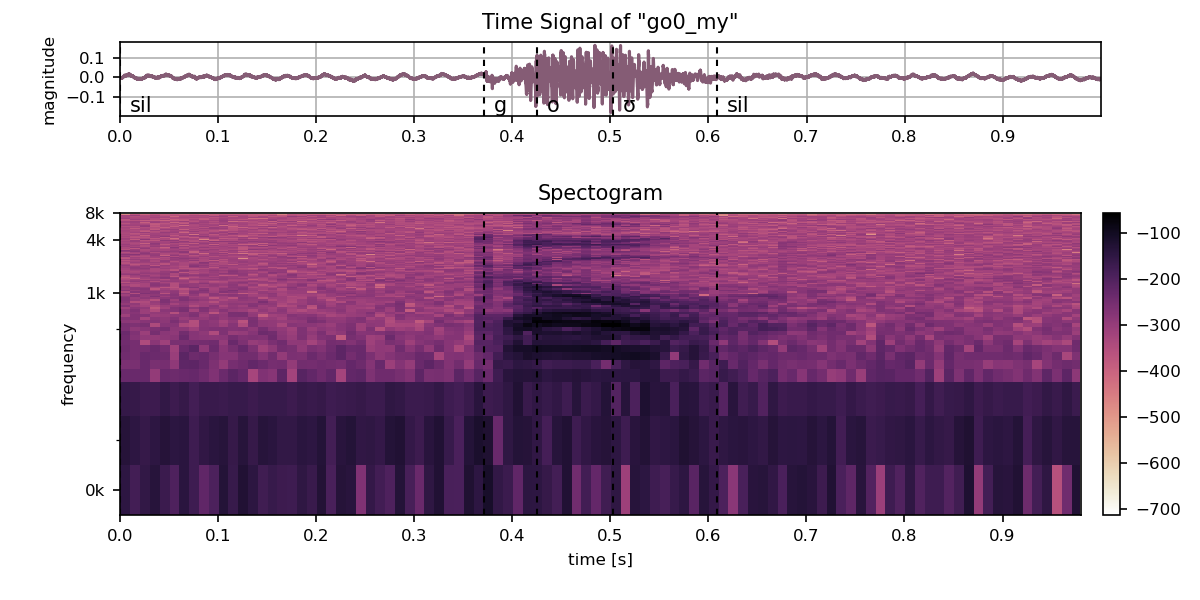
\includegraphics[width=0.45\textwidth]{./3_signal/figs/signal_spec-log_go0_my}}
  \caption{Spectrogram logarithmic scaled.}
  \label{fig:signal_spec_log_examples}
\end{figure}
\FloatBarrier
\noindent

Now it is possible to see some interesting structures and movements in the spectrograms in the frequency axis over time.
Still it is possible to improve the visualization of the spoken command words with a better compression scheme, such as the Mel Frequency Cepstral Coefficients, explained in the next section.
% --
% mfcc

\section{Mel Frequency Cepstral Coefficients}\label{sec:signal_mfcc}
Most commonly the Mel Frequency Cepstral Coefficients (MFCC) are used as input features for Neural Network classifications tasks of audio data.
It is described why they are good features and how they can be visualized to understand them better.

\begin{figure}[!ht]
  \centering
    \subfigure[left]{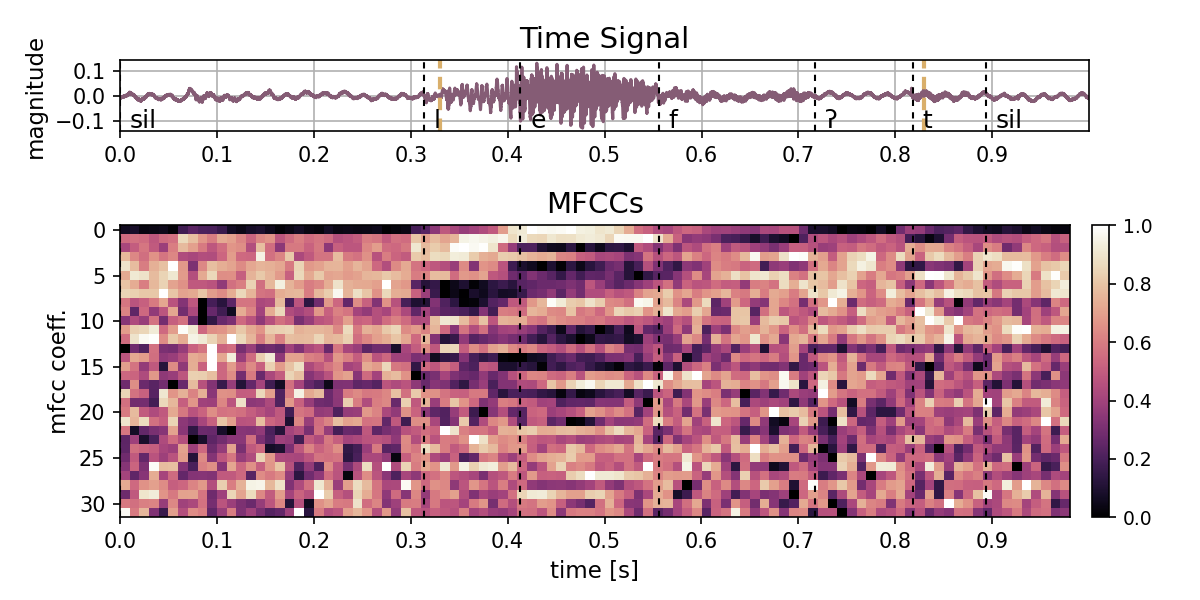
\includegraphics[width=0.45\textwidth]{./3_signal/figs/signal_mfcc_left0_my}}
    \subfigure[right]{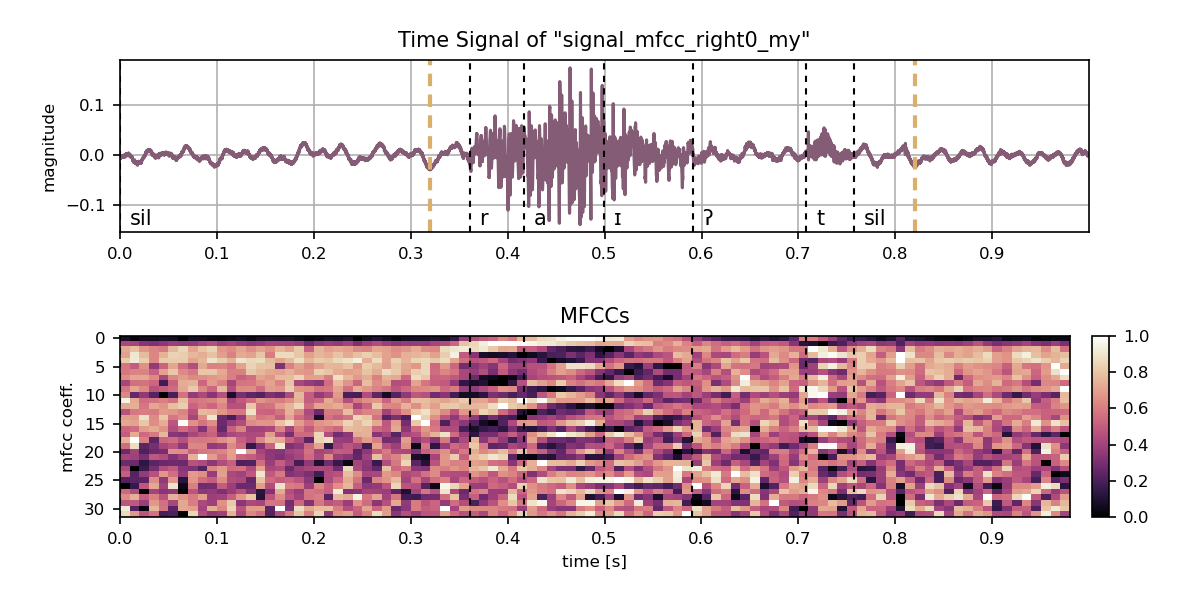
\includegraphics[width=0.45\textwidth]{./3_signal/figs/signal_mfcc_right0_my}}
    \subfigure[up]{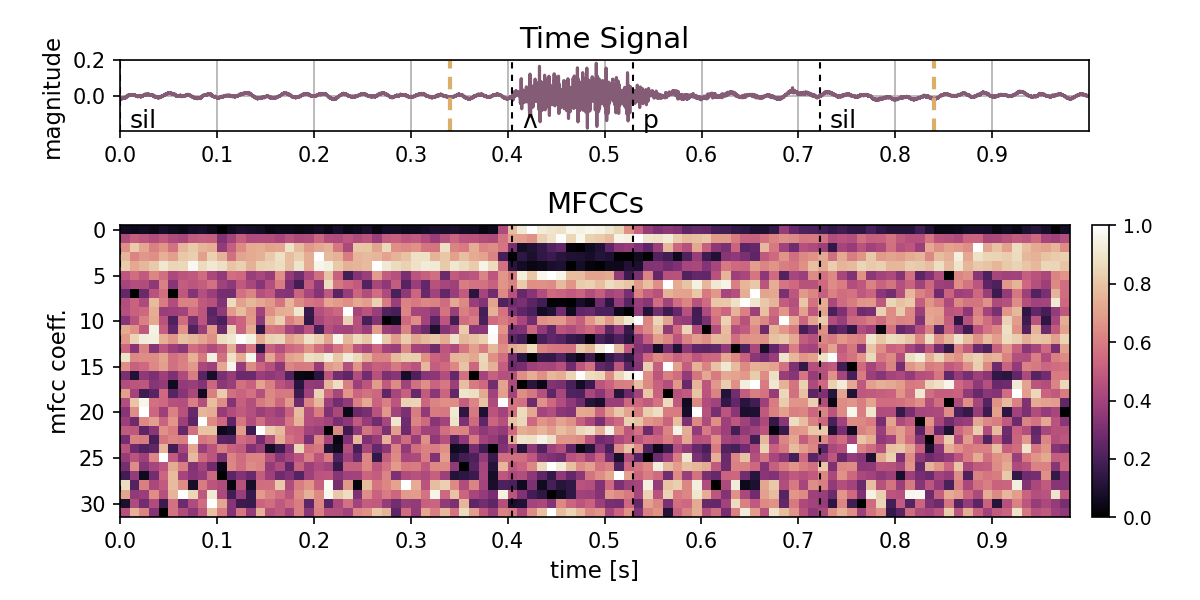
\includegraphics[width=0.45\textwidth]{./3_signal/figs/signal_mfcc_up0_my}}
    \subfigure[down]{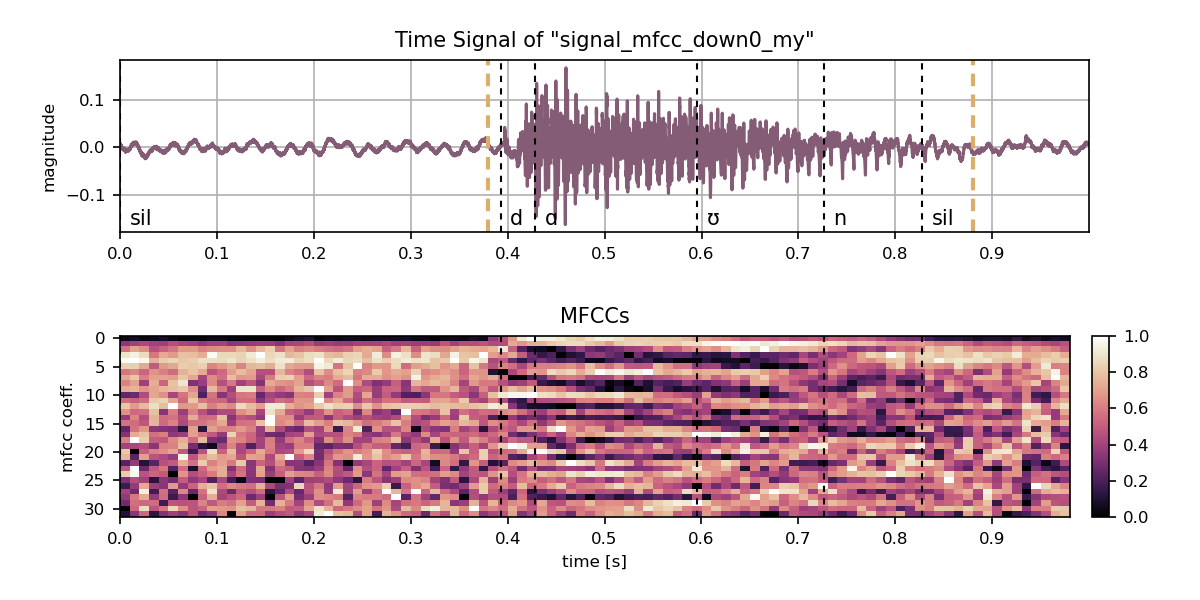
\includegraphics[width=0.45\textwidth]{./3_signal/figs/signal_mfcc_down0_my}}
    \subfigure[go]{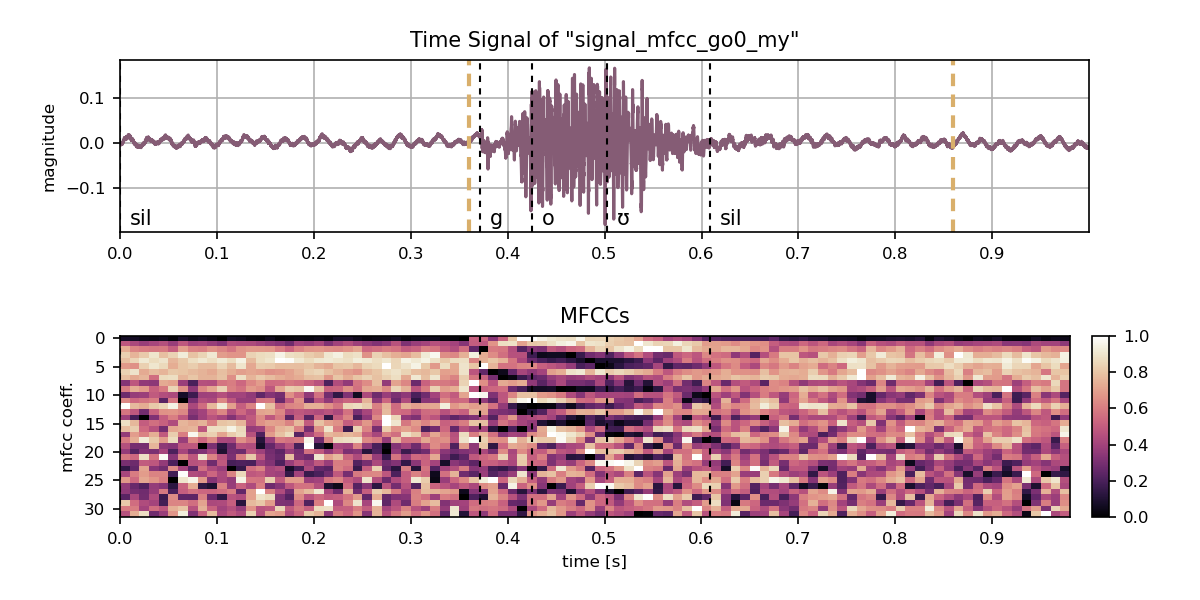
\includegraphics[width=0.45\textwidth]{./3_signal/figs/signal_mfcc_go0_my}}
  \caption{MFCC visualized with frame-based normalization.}
  \label{fig:signal_mfcc_examples}
\end{figure}
\FloatBarrier
\noindent

\subsection{The Idea behind}
To comprehend the success and wide use of MFCCs features in Neural Networks and other machine learning applications, it is necessary to understand its processing scheme:
Raw audio samples are transformed into the frequency domain with the Short-Time Fourier Transform (STFT).
Afterwards the power spectrum of the STFT is segmented in frequency bands (along the frequency dimension) done by a filter bank.
The filter bands are spaced in equidistant mel frequencies,
where the term mel frequencies is referred to the non-linear relationship between the mel and frequency scale.
The mel scale was developed in psychoacoustic experiments, where researchers found out, that high frequency sounds are perceived lower by humans, than they actual are (in musical hearing). For instance, in the musical sense an octave is the doubling of the frequency, but for human hearing it is strongly different and frequency doubling is not enough so that the same pitch is perceived.
This effect usually becomes imminent over \SI{500}{\hertz}.
As conclusion the mel scale is suited human hearing perception and taking equidistant mel bands is a reasonable decision.
In the following a logarithmic scaling in the value space of the power spectrum is done, which is also related to human hearing.
The last step is not that straight forward, but is a technique widely used in image processing, called the Discrete Cosine Transform (DCT).
It is only to mention that is some kind of decorrelation process, so that different filter bands are mixed together.

This processing steps seem rather complicated in the beginning, but are in fact nothing else but consecutive steps of appropriate scaling and data compression.
It is to mention that Neural Networks usually are able to handle large amounts of input features, but it is always preferable to decrease the input size, such that the model size of the Neural Network can be decreased same-wise.
Therefore it becomes more clear, why frequencies are put into certain frequency bands, are log scaled and as last step decorrelated with a method like the DCT.

\subsection{Processing Pipeline in detail}
The frequency spectrum is spitted into filter bands, done by triangular window functions.
Those window functions must have a fixed length on the mel space (equidistant mel bands), that results in different spacings in
the frequency space.
The mel - frequency relation can be approximated with:
\begin{equation}\label{eq:signal_mfcc_mel}
  m(f) = 2595 \cdot \log_{10} \left(1 + \frac{f}{700} \right) 
\end{equation}
where $m$ is the result in mel scale as function of the frequency $f$.
The mel scale plotted against the frequency scale is illustrated in \rfig{signal_mfcc_mel_scale}
\begin{figure}[!ht]
  \centering
  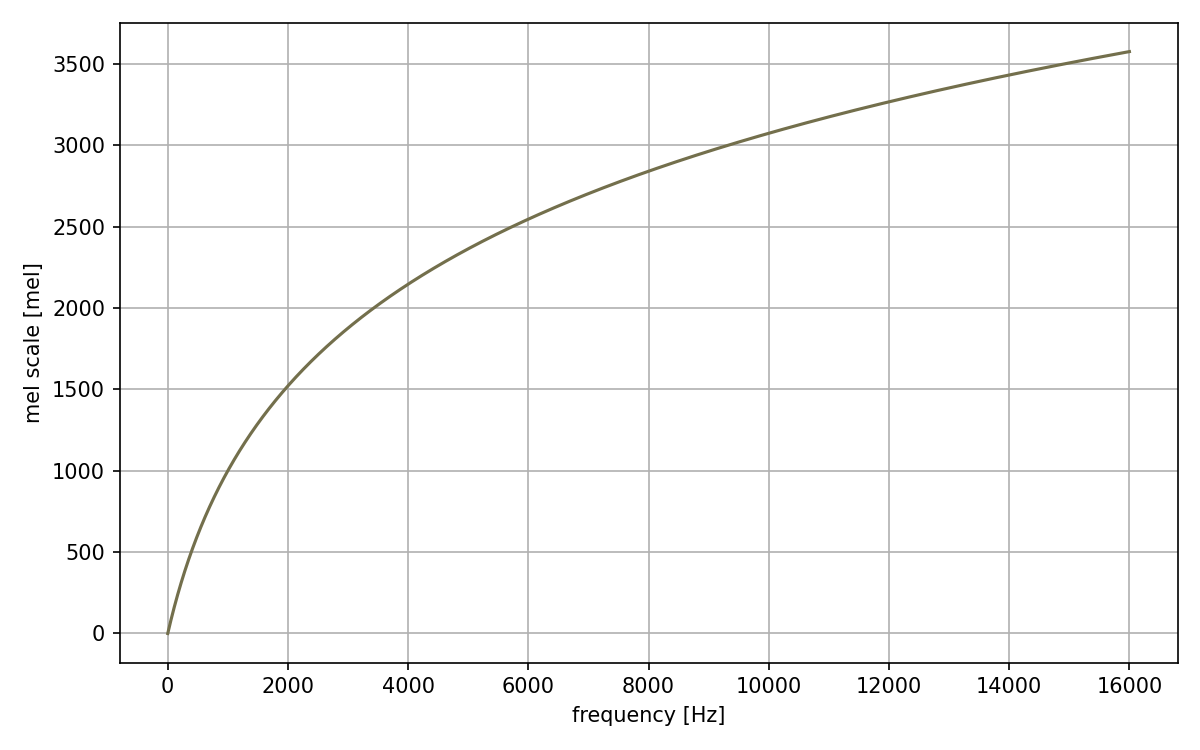
\includegraphics[width=0.40\textwidth]{./3_signal/figs/signal_mfcc_mel_scale}
  \caption{Mel scale as function of the frequency in a range of [0, \SI{16}{\kilo\hertz}].}
  \label{fig:signal_mfcc_mel_scale}
\end{figure}
\FloatBarrier
\noindent


The mel and frequency window functions are shown in \rfig{filter_bands}.
\begin{figure}[!ht]
  \centering
  \subfigure[mel space]{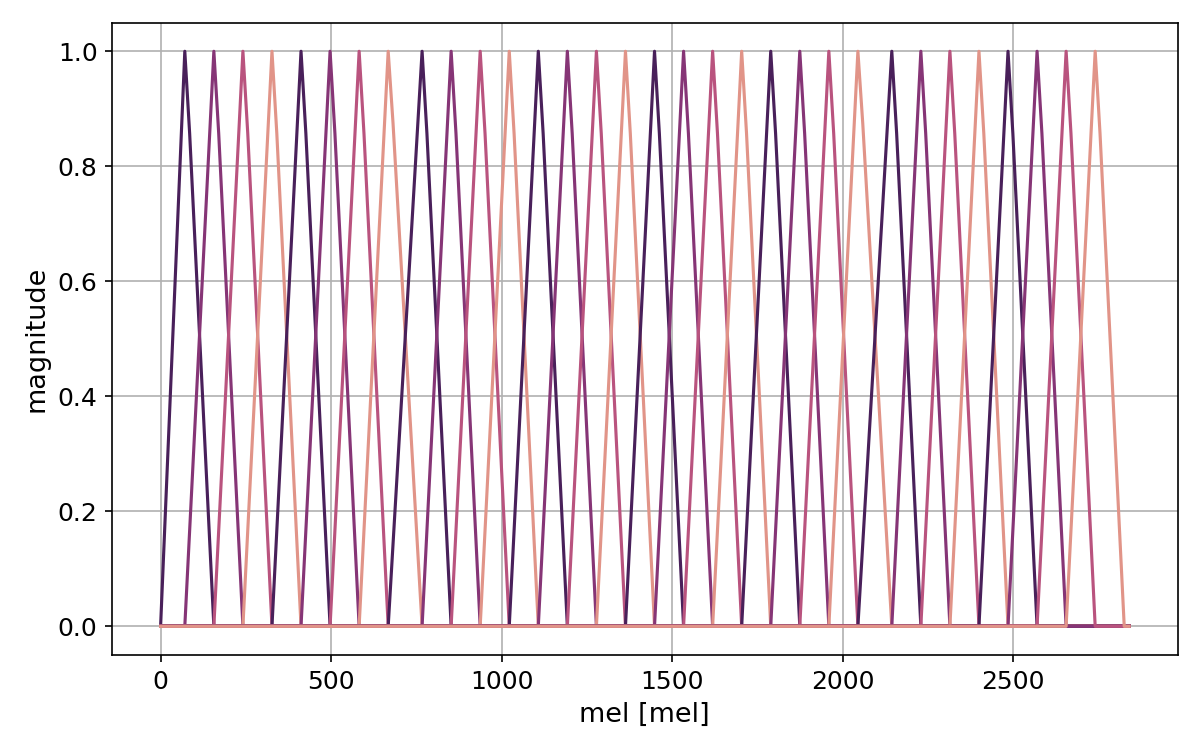
\includegraphics[width=0.40\textwidth]{./3_signal/figs/signal_mfcc_weights_mel}}
  \quad
  \subfigure[frequency space]{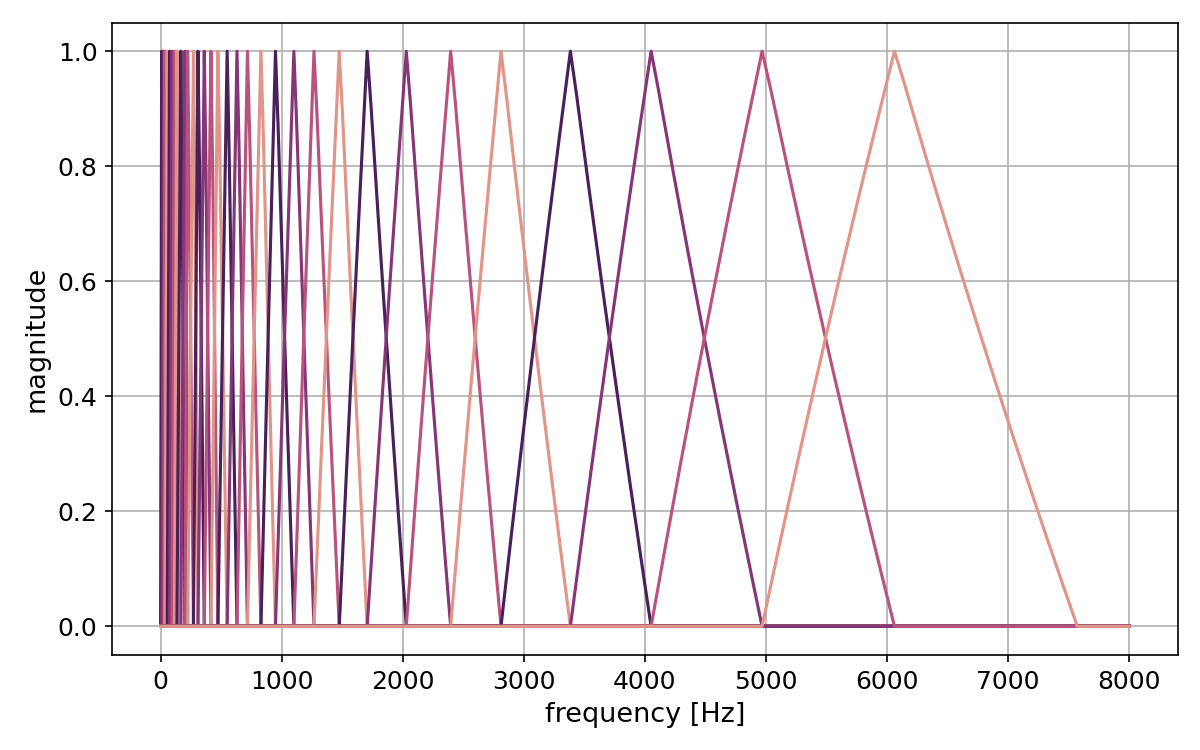
\includegraphics[width=0.40\textwidth]{./3_signal/figs/signal_mfcc_weights_f}}
  \caption{Equidistant mel filter bands with a total number of 32 bands.}
  \label{fig:filter_bands}
\end{figure}
\FloatBarrier
\noindent

The DCT is similar to the Fourier Transform and projects the input signal to a set of basis functions. 
These Basis functions are illustrated in \rfig{dct}
\begin{figure}[!ht]
  \centering
  \subfigure[DCT with continuous color scheme]{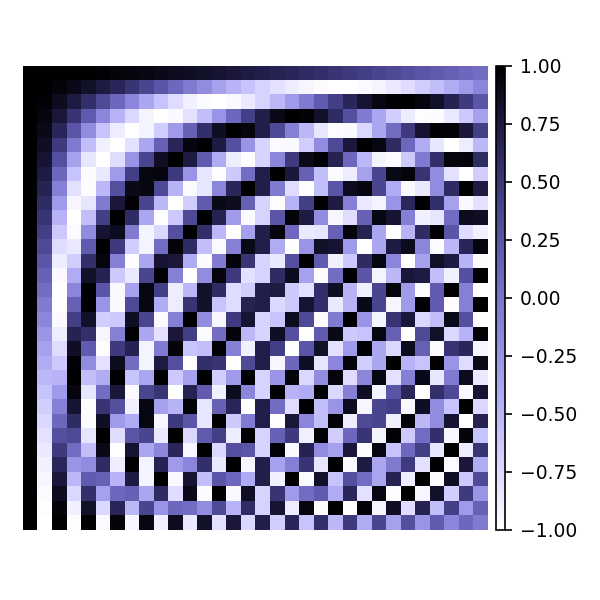
\includegraphics[width=0.40\textwidth]{./3_signal/figs/signal_mfcc_dct}}
  \quad
  \subfigure[DCT with diverging color scheme]{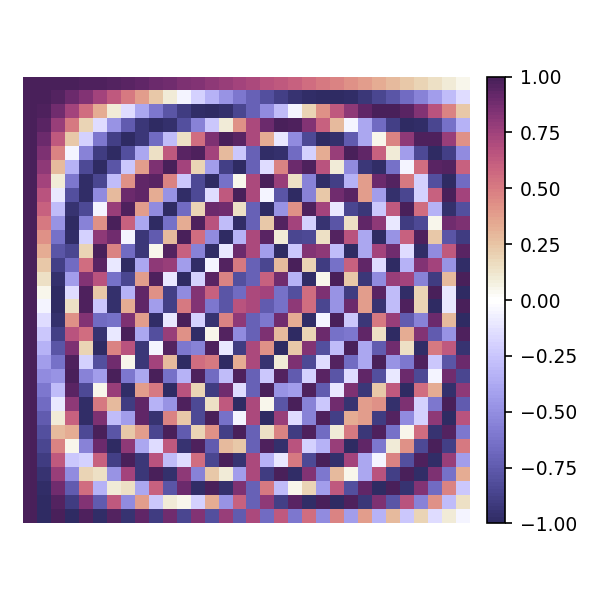
\includegraphics[width=0.40\textwidth]{./3_signal/figs/signal_mfcc_dct-div}}
  \caption{DCT matrix with 32 basis functions illustrated with a continuous and a diverging color scheme.}
  \label{fig:dct}
\end{figure}
\FloatBarrier
\noindent


\subsection{MFCC Feature Usage and Enhancement}
After the MFCCs are computed, they can be used as input features for Neural Networks. 
The important Question here is whether an feature enhancement can be done and if all those computed features are necessarily and meaningful for the training and evaluation success of Neural Networks. Usually not all MFCC coefficients are used as inputs, this is merely done to reduce the computational cost in case the accuracy does not suffer from it.
A good application is to compute 32 MFCC features (with 32 equidistant Mel filter bands) and use only the first 12 of them as inputs.
Further it is also possible to compute derivatives (in the time domain) of MFCC features, denoted as Deltas. 
Those derivatives are simple computed as frame difference of the MFCCs.
A second derivative of MFCC features, known as Double Deltas, are then the frame differences of the Deltas.
At last an energy feature can be computed from each of the MFCCs, Deltas and Double Deltas, each by its own and added to the feature vectors.
Those feature vectors can then be simply stacked at top of each other and used as feature inputs.
In this thesis the feature vectors are stacked as following:
\begin{enumerate}
    \item 12 MFCCs
    \item 1 Energy feature of the 12 MFCCs
    \item 12 Deltas
    \item 1 Energy feature of the 12 Deltas
    \item 12 Double Deltas
    \item 1 Energy feature of the 12 Double Deltas
\end{enumerate}
Which sums up to a 39-dimensional feature vector.

\subsection{Visualisation of MFCC features}
A good visualisation of MFCC features is the best way to understand them.
With this thought in mind, much time was spent to create a fitting visual representation of the MFCC features, but this was not an easy task.
MFCCs are not well intended for visualisations, since their individual coefficients value space, can be strongly different from each other.
For example, the first coefficient equals a summation of all filter bands and is therefore some kind of energy measure over all bands, while the other coefficients are weighted sum combinations of the filter bands.
This alone yields in totally different value spaces and value spaces should not differ that much, when features should be represented with colors.
Further it is to mention, that most of the signal energy will be in the lower frequency bands, which also impacts the value space of the individual coefficients a lot.
To show this difference in value space in a negative example in practise, the MFCCs of the self-recorded speech command waveform \enquote{left0.wav} is shown in \rfig{left0_mfcc_only}.

\begin{figure}[!ht]
  \centering
    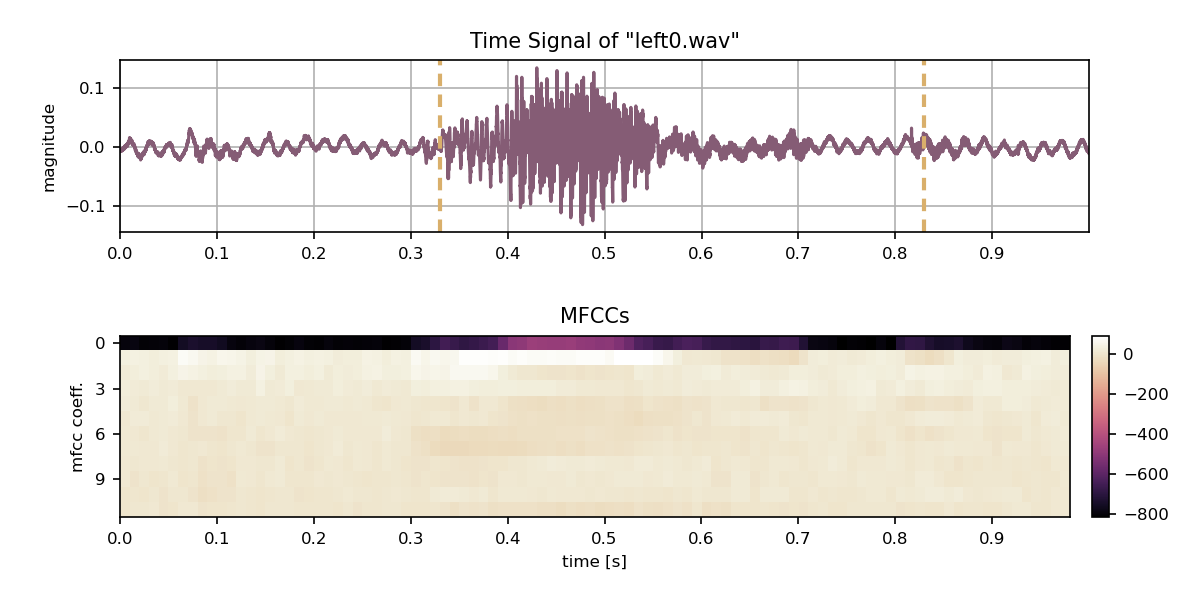
\includegraphics[width=0.75\textwidth]{./3_signal/figs/signal_mfcc_left0_mfcc_only.png}
  \caption{Bad visualisation of the 12 MFCCs features extracted from \enquote{left0.wav}.}
  \label{fig:left0_mfcc_only}
\end{figure}
\FloatBarrier
\noindent
Not much structure of the MFCCs can be seen here, due to the vast value difference of the first coefficient. At least the first coefficient shows, where the center of signal energy is placed on the time scale, but other than that, this visualisation is worthless.
Another very bad visualisation is shown by computing the 39 MFCC feature vectors (with Deltas, Double Deltas and Energies) in \rfig{left0_no_order}.

\begin{figure}[!ht]
  \centering
    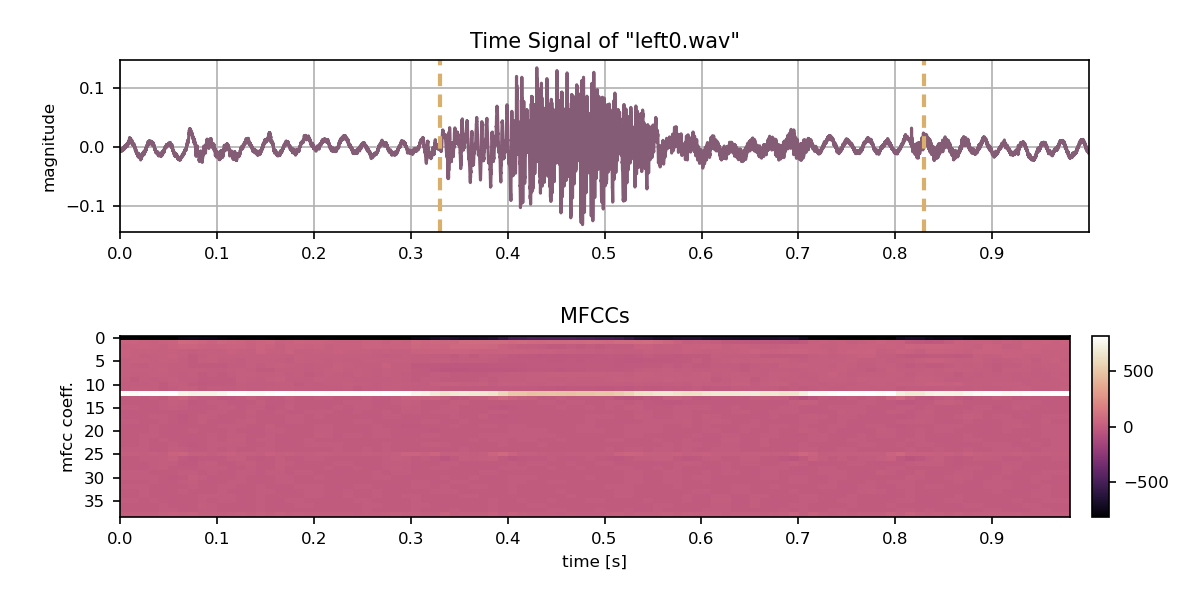
\includegraphics[width=0.75\textwidth]{./3_signal/figs/signal_mfcc_left0_no_order_norm0.png}
  \caption{Very bad visualisation of 39 MFCC features extracted from \enquote{left0.wav}.}
  \label{fig:left0_no_order}
\end{figure}
\FloatBarrier
\noindent
There appears an even greater gap of different value spaces and even less is seen.
One very easy solution is to show the features in different value groups. For instance the first coefficient and its deltas is in one group, the other coefficients in another and the deltas and energies are separated as well in own groups. Now we actually can see some structure in the visualisations, shown in \rfig{left0_order}.

\begin{figure}[!ht]
  \centering
    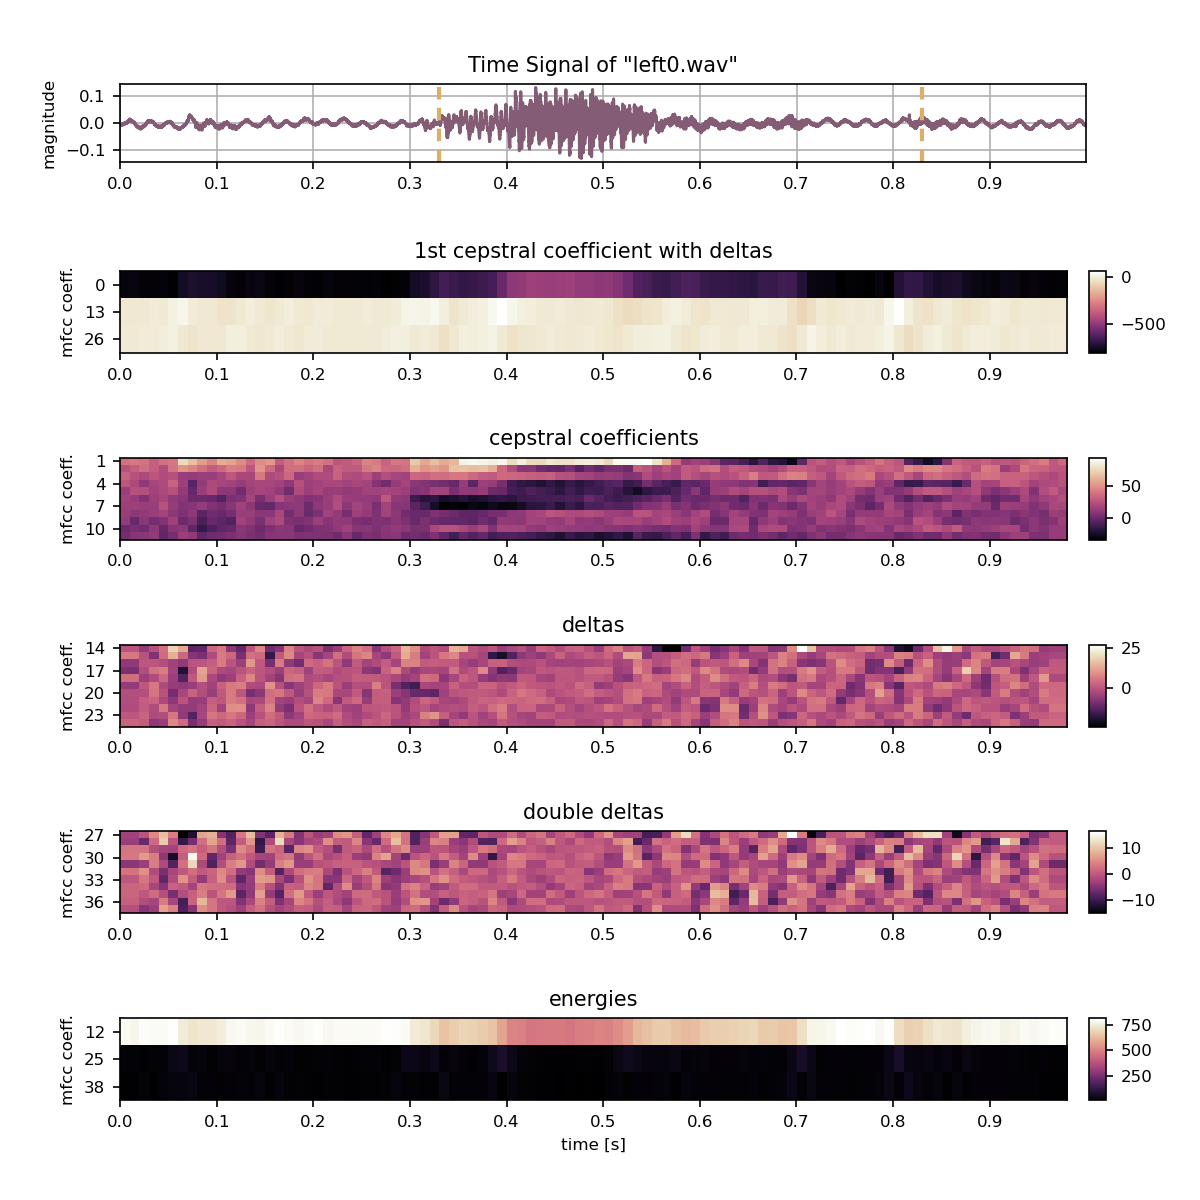
\includegraphics[width=0.75\textwidth]{./3_signal/figs/signal_mfcc_left0_norm0.png}
  \caption{Good visualisation of 39 MFCC features extracted from \enquote{left0.wav} with own value groupings.}
  \label{fig:left0_order}
\end{figure}
\FloatBarrier
\noindent
Another way to improve the visualisation is to normalize the feature vectors over their each own frame dimension with the infinity norm. This will yield a value space of $[0, 1]$ for each feature vector. With this, the visualisation of the 39 MFCC of \enquote{left0.wav} is shown in \rfig{left0_order},

\begin{figure}[!ht]
  \centering
    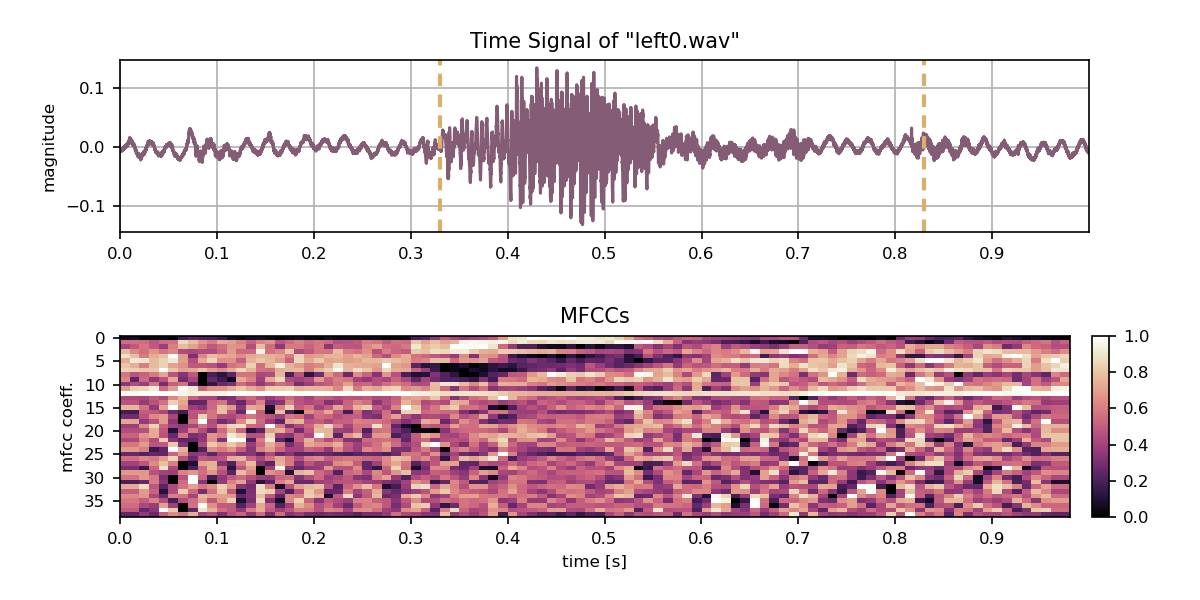
\includegraphics[width=0.75\textwidth]{./3_signal/figs/signal_mfcc_left0_no_order_norm1.png}
  \caption{Normalisation of 39 MFCC features extracted from \enquote{left0.wav}.}
  \label{fig:left0_no_order_norm1}
\end{figure}
\FloatBarrier
\noindent
or in an even better one shown in \rfig{left0_order_norm1}.

\begin{figure}[!ht]
  \centering
    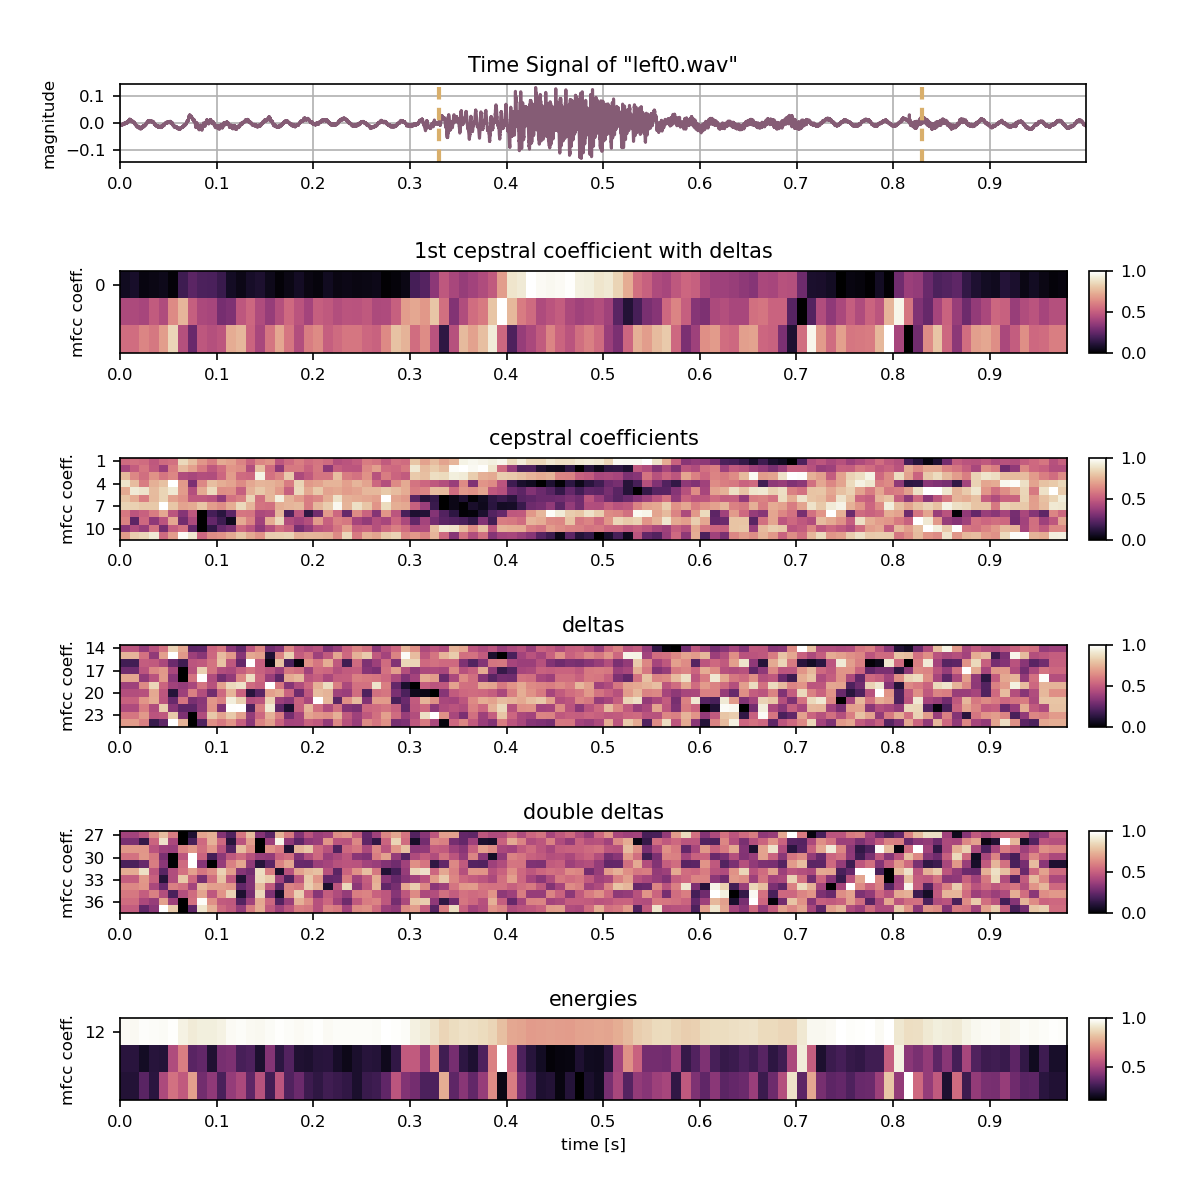
\includegraphics[width=0.75\textwidth]{./3_signal/figs/signal_mfcc_left0_order_norm1.png}
  \caption{Normalisation of 39 MFCC features extracted from \enquote{left0.wav} with groups.}
  \label{fig:left0_order_norm1}
\end{figure}
\FloatBarrier
\noindent
As conclusion, the normalisation in the frame space is an interesting aspect to improve the visualisation of the MFCC features, 
specifically for the cepstral coefficients and the energy features (not the deltas).
Exactly this nice representation was motivating to explore normalisation of feature for Neural Network inputs.
However this is a very crucial thing to do. A normalisation relatives important structures within the feature space and it cannot really be answered if this is a good thing or not.
One more research question arises here: Is it possible to use normalisation for the features as inputs to Neural Networks and what are the results to the accuracy and training of the models.

